
%(BEGIN_QUESTION)
% Copyright 2013, Tony R. Kuphaldt, released under the Creative Commons Attribution License (v 1.0)
% This means you may do almost anything with this work of mine, so long as you give me proper credit

Calculate the mass of 3.4 moles of glutaric anhydride, the ``line drawing'' for this organic molecule shown here:

$$\includegraphics[width=15.5cm]{i02649x01.eps}$$

\underbar{file i02649}
%(END_QUESTION)





%(BEGIN_ANSWER)

Converting the line drawing into a molecular formula, we get C$_{11}$H$_{10}$O$_{3}$.  Remember that the general rule for interpreting line drawings is that every vertex or intersection of lines marks the location of one carbon atom having four bonds, and that any bonds not shown are bonds to hydrogen atoms.  The molecular weight for this formula is approximated as follows:

$$(12)(11) + (1)(10) + (16)(3) = 190 \hbox{ amu} = 190 \hbox{ grams per mole glutaric anhydride}$$

\vskip 10pt

Calculating mass given the molar quantity of this compound:

$$\left(3.4 \hbox{ mol glutaric anhydride} \over 1 \right) \left(190 \hbox{ g} \over \hbox{ mol glutaric anhydride}\right) = 646 \hbox{ g}$$


%(END_ANSWER)





%(BEGIN_NOTES)


%INDEX% Chemistry, stoichiometry: moles

%(END_NOTES)


